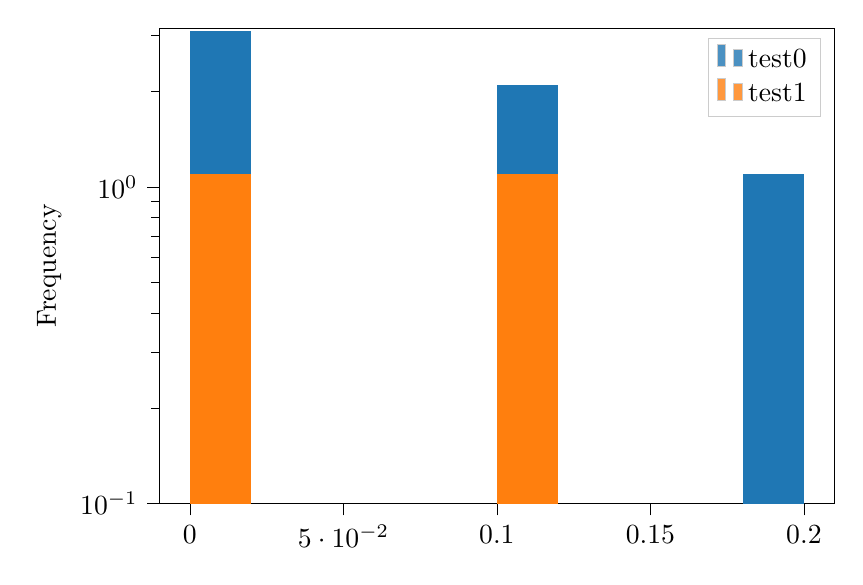
\begin{tikzpicture}

\definecolor{darkgray176}{RGB}{176,176,176}
\definecolor{darkorange25512714}{RGB}{255,127,14}
\definecolor{lightgray204}{RGB}{204,204,204}
\definecolor{steelblue31119180}{RGB}{31,119,180}

\begin{axis}[
height=3in,
legend cell align={left},
legend style={fill opacity=0.8, draw opacity=1, text opacity=1, draw=lightgray204},
log basis y={10},
tick align=outside,
tick pos=left,
width=4in,
x grid style={darkgray176},
xmin=-0.01, xmax=0.21,
xtick style={color=black},
y grid style={darkgray176},
ylabel={Frequency},
ymin=0.1, ymax=3.1694019,
ymode=log,
ytick style={color=black}
]
\draw[draw=none,fill=steelblue31119180] (axis cs:1.7347235e-18,0.1) rectangle (axis cs:0.02,3.1);
\addlegendimage{ybar,ybar legend,draw=none,fill=steelblue31119180}
\addlegendentry{test0}

\draw[draw=none,fill=steelblue31119180] (axis cs:0.02,0.1) rectangle (axis cs:0.04,0.1);
\draw[draw=none,fill=steelblue31119180] (axis cs:0.04,0.1) rectangle (axis cs:0.06,0.1);
\draw[draw=none,fill=steelblue31119180] (axis cs:0.06,0.1) rectangle (axis cs:0.08,0.1);
\draw[draw=none,fill=steelblue31119180] (axis cs:0.08,0.1) rectangle (axis cs:0.1,0.1);
\draw[draw=none,fill=steelblue31119180] (axis cs:0.1,0.1) rectangle (axis cs:0.12,2.1);
\draw[draw=none,fill=steelblue31119180] (axis cs:0.12,0.1) rectangle (axis cs:0.14,0.1);
\draw[draw=none,fill=steelblue31119180] (axis cs:0.14,0.1) rectangle (axis cs:0.16,0.1);
\draw[draw=none,fill=steelblue31119180] (axis cs:0.16,0.1) rectangle (axis cs:0.18,0.1);
\draw[draw=none,fill=steelblue31119180] (axis cs:0.18,0.1) rectangle (axis cs:0.2,1.1);
\draw[draw=none,fill=darkorange25512714] (axis cs:1.7347235e-18,0.1) rectangle (axis cs:0.02,1.1);
\addlegendimage{ybar,ybar legend,draw=none,fill=darkorange25512714}
\addlegendentry{test1}

\draw[draw=none,fill=darkorange25512714] (axis cs:0.02,0.1) rectangle (axis cs:0.04,0.1);
\draw[draw=none,fill=darkorange25512714] (axis cs:0.04,0.1) rectangle (axis cs:0.06,0.1);
\draw[draw=none,fill=darkorange25512714] (axis cs:0.06,0.1) rectangle (axis cs:0.08,0.1);
\draw[draw=none,fill=darkorange25512714] (axis cs:0.08,0.1) rectangle (axis cs:0.1,0.1);
\draw[draw=none,fill=darkorange25512714] (axis cs:0.1,0.1) rectangle (axis cs:0.12,1.1);
\draw[draw=none,fill=darkorange25512714] (axis cs:0.12,0.1) rectangle (axis cs:0.14,0.1);
\draw[draw=none,fill=darkorange25512714] (axis cs:0.14,0.1) rectangle (axis cs:0.16,0.1);
\draw[draw=none,fill=darkorange25512714] (axis cs:0.16,0.1) rectangle (axis cs:0.18,0.1);
\draw[draw=none,fill=darkorange25512714] (axis cs:0.18,0.1) rectangle (axis cs:0.2,0.1);
\end{axis}

\end{tikzpicture}
